\section{Resolución Problema 3}
Dada una circunferencia con centro en el punto
C con coordenadas (x1, y1) y radio r, evaluar si
un punto T con coordenadas (x2, y2) esta dentro
del área de la circunferencia.


\subsection{\textbf{Descripción del problema:}}
El problema implica calcular la distancia de dos puntos 
Dónde el punto C y el punto T pueden ser definidos en el plano cartesiano (X,Y) y R es definidas asía los cuatro ejes, además debemos tomar en cuenta que el punto T se puede encontrar dentro o fuera de la circunferencia 


\subsection{\textbf{Definición de solución:}}
En el primer segmento considerando las variables X1,X2 y Y1,Y2 se plantea la siguiente solución se emplea la formula: distancia:
\\
${Distancia} = \sqrt{{(x_2 - x_1)^2 + (y_2 - y_1)^2}}$,
\\
Con esta formula se calcula la distancia entre los dos puntos  \texttt{(C y T)}.Posterior mente se verifica que el radio ingresado sea positivo, en dado caso de que el radio sea negativo se utilizara la formula: Radio*-1; con esta formula se convierte el radio negativo a positivo,finalmente verificamos que el punto se encuentre dentro de la circunferencia utilizando el radio . 
\\
-Observamos como se plasma en el plano cartesiano utilizando la formula de la distancia
\begin{figure}[H]
    \centering
    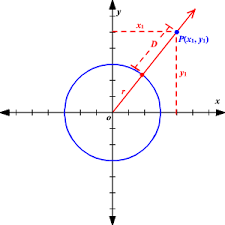
\includegraphics[width = 5 cm]{LaTeX/latex-imagenes/Imagen7.png}
    \caption{Gráfica del programa}
    \label{fig:imagen7}
\end{figure}


\subsection{\textbf{Diseño de la solución:}}
\begin{enumerate}[label=\textbf{\arabic*.}]

  \item Considerando las variables X,Y de cada punto calcula la distancia entre los dos puntos utilizando la siguiente formula: {distancia} = \sqrt{{(x_2 - x_1)^2 + (y_2 - y_1)^2}}.

  \item  Considerando que la variable r sea positiva se procedera al siguiente paso, de lo contrario se aplicara la siguiente ecuacion r*-1.
  \item considerando que la distancia sea menor al radio se puede decir que el punto T se encuentra dentro de la circunferencia, de lo contrario se considera que el punto se encuentra fuera de la circunferencia. 
  \\
  A continuación veremos el diagrama de flujo que fue la base para el desarrollo del programa.
\end{enumerate}
\begin{figure}[H]
    \centering
    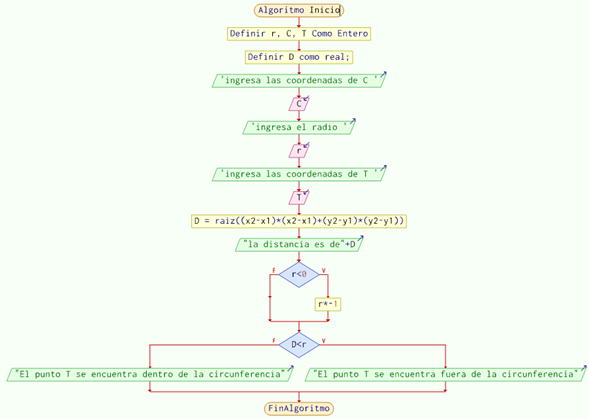
\includegraphics[width = 8 cm]{LaTeX/latex-imagenes/diagramaz.png}
    \caption{Diseño del programa}
    \label{fig:imagen7}
\end{figure}


\subsection{\textbf{Desarrollo de la solución:}}
A continuación, se muestra el código en Java para calcular la distancia entre dos puntos y verificar si se encuentran dentro de una circunferencia:


  \\
  \\
  
        Primero se solicita al usuario las coordenadas del punto C (x1,y1)
       \begin{javaCode}
        Scanner dato = new Scanner(System.in);
        System.out.print("Ingrese las coordenada del punto C primero x1: ");
        int x1 = dato.nextInt();
        System.out.print("Ingrese las coordenada del punto C despues  y1: ");
        int y1 = dato.nextInt();
         \end{javaCode}
         se solicita el radio de la circunferencia
       
        \begin{javaCode}
        System.out.println("Ingrese el radio de la circunferencia: ");
        int radio = dato.nextInt();
         \end{javaCode}
         
        solicitamos al usuario las coordenadas del punto T (x2,y2)
       \begin{javaCode}
        System.out.print("Ingrese las coordenada del punto T X2: ");
        int x2 = dato.nextInt();
        System.out.print("Ingrese las coordenada del punto T Y2: ");
        int y2 = dato.nextInt();
        \end{javaCode}
         Se realiza el cálculo  la distancia entre el punto C y el punto T con ayuda de la formula antes mencionada.
        \begin{javaCode}
        double distancia = Math.sqrt((x2 - x1) * (x2 - x1) + (y2 - y1) * (y2 - y1));
        \end{javaCode}
         Se imprime el resultado del calculo de la distancia.
          \begin{javaCode}
         System.out.println("la distancia es de "+distancia);
          \end{javaCode}
       
        Se verifica si el radio es positivo o negativo, si es negativo lo pasamos a positivo
         \begin{javaCode}
        int radio2=radio*-1;
\end{javaCode}
         Se calcula, si la distancia resulta menor o igual al radio entonces el punto T se encontrara dentro de la circunferencia, de lo contrario el punto T se encontrara fuera de la circunferencia .    
       
        \begin{javaCode}
                    if(radio<0){
            
        
        int radio2=radio*-1;
        if (distancia <= radio2) {
            System.out.println("El punto T está dentro de la circunferencia");
        } else {
            System.out.println("El punto T no está dentro de la circunferencia");
        }
        }
        
       if(radio>0){
           
       
            if (distancia <= radio) {
            System.out.println("El punto T está dentro de la circunferencia");
        } else {
            System.out.println("El punto T no está dentro de la circunferencia");
        }
    }
    
    
    }
    
}
    \end{javaCode}

    
\subsection{\textbf{Depuración y pruebas:}}
Se realizaron 5 pruebas al programa para validar su funcionamiento, a continuación veremos los siguientes resultados 



   \begin{figure}[H]
    \centering
    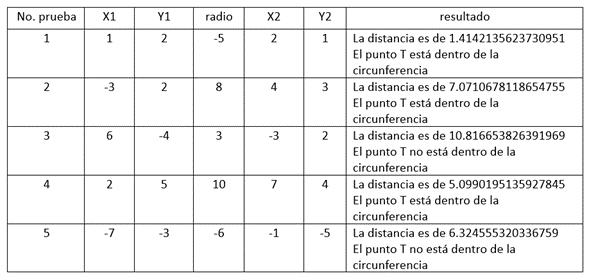
\includegraphics[width = 11 cm]{LaTeX/latex-imagenes/tabla de prueba.png}
    \caption{Tabla de pruebas}
    \label{fig:Grafica de la distancia de dos puntos }
\end{figure}